\documentclass[a4paper, 12pt]{article}
%\usepackage[utf8]{inputenc}
\usepackage{appendix}
\usepackage{listings}
\usepackage{color}
\usepackage{xcolor}
\usepackage{float}
\usepackage[british]{babel}
\usepackage{amsmath}
\usepackage{amsfonts}
\usepackage{amssymb}
\usepackage{amsthm}
%\usepackage{amsrefs}
\usepackage{enumerate}
\usepackage{graphicx}
\usepackage{caption}
\usepackage{subcaption}
\usepackage{url}
\usepackage[round]{natbib}
\usepackage[all]{xy}
\usepackage{tikz}
\usepackage{hyperref}
\usepackage[percent]{overpic}
\usepackage[printwatermark]{xwatermark}
\usepackage{epstopdf}
\usepackage{fancyvrb}
\usepackage{longtable}
\usepackage{wasysym}
%\usepackage{multicol}
\usepackage{pgfplots}
%\usepackage{newtxtext,newtxmath}
%\newwatermark[allpages,color=red!20,angle=45,scale=4,xpos=0,ypos=0]{DRAFT}

%\usepackage{antpolt}
%\usepackage[T1]{fontenc}
%\usepackage{tocloft}
\usepackage{selinput}
\SelectInputMappings{
  adieresis={ä},
  edieresis={ë},
  idieresis={ï},
  udieresis={ü},
  eacute={é},
}

\newcommand{\widefigwidth}{\textwidth}
\newcommand{\mgraphheight}{.21\textheight}

\usetikzlibrary{positioning}

\definecolor{MidnightBlue}{RGB}{11,28,121}
\definecolor{dkgreen}{rgb}{0,0.6,0}
\definecolor{mauve}{rgb}{0.58,0,0.82}

\newcommand{\citeneed}{{\color{red} [citation needed] }}
\newcommand{\citepos}{{\color{orange} [citation needed?] }}
\newcommand{\todo}[1]{{\color{red} TODO:} {\color{dkgreen} #1}}
\newcommand{\ennl}[1]{{\color{red} \it [TL: #1]}}

\newcommand{\Python}{\texttt{Python}}

\renewcommand{\thefigure}{\arabic{section}.\arabic{figure}}

\newcommand{\mat}[1]{\left(\begin{matrix} #1 \end{matrix} \right)}
\newcommand{\HRule}{\rule{\linewidth}{0.5mm}}
%\renewcommand{\cftdot}{}
%\renewcommand{\cftsecleader}{\cftdotfill{\cftdotsep}}
\setcounter{tocdepth}{3}

\usepackage{tikz}
\usetikzlibrary{shapes,arrows}

\floatstyle{ruled}
\newfloat{example}{htb}{lop}
\floatname{example}{Example}
\newfloat{codeblok}{htb}{lop}
\floatname{codeblok}{Codeblok}

%\newcommand{\citep}[1]{\cite{#1}}\newcommand{\citet}[1]{\cite{#1}}
\renewcommand{\cite}[1]{\citep{#1}}

\renewcommand{\lstlistingname}{Codeblok}
\lstdefinestyle{lstjava}{
language=Java,
numbers=left,
numberstyle=\tiny\color{red},
stepnumber=5,
numbersep=5pt,
tabsize=2,
breaklines=true,
keywordstyle=\color{MidnightBlue},
commentstyle=\color{dkgreen},
stringstyle=\color{mauve},
morekeywords={}
}
\lstdefinestyle{lstmatlab}{
language=Matlab,
numbers=left,
numberstyle=\tiny\color{red},
stepnumber=5,
numbersep=5pt,
tabsize=2,
breaklines=true,
keywordstyle=\color{MidnightBlue},
commentstyle=\color{dkgreen},
stringstyle=\color{mauve},
morekeywords={linreg,linregquad,logreg,ones,repmat}
}
\lstnewenvironment{lstmat}{
\lstset{style=lstmatlab}}{}

\lstnewenvironment{lstsource}{
\lstset{
language=C,
breaklines=true,
showspaces=false,
showstringspaces=false,
showtabs=false,
morekeywords={}
}}{}

\lstdefinestyle{lstcpp}{
language=C++,
numbers=left,
numberstyle=\tiny\color{red},
stepnumber=5,
numbersep=5pt,
tabsize=2,
breaklines=true,
keywordstyle=\color{MidnightBlue},
commentstyle=\color{dkgreen},
stringstyle=\color{mauve},
morekeywords={}
}


\title{Automatic Plastic Soup Solver}
\author{Ysbrand Galama \\ 10262067}
\date{\today}

\begin{document}
\pagenumbering{gobble}
\begin{center}
\huge \bf Automatic Plastic Soup Solver
\end{center}
\noindent
\hfill \today\\
{\bf
Project: Visual Recognition to Conserve Nature\\
Supervisor: Thomas Mensink\\
Applicant: Ysbrand Galama, 10262067
}

\noindent
% 0. Geef je tender een titel: Automatic Plastic Soup Solver (of zo iets :-) )
% 1. Een paragraaf over de plastic-soup (voeg 1/2 plaatjes toe, ook over de omvang van het probleem).
% 2. Een (kleine) paragraag over Saraswater, met hun specifieke probleem: het aansturen van schepen om plastic op te ruimen.
% 3. Een paragraaf over je dataset, zeg dat die al gelabeled is (Ook hier: voeg plaatjes toe).
% 4. Dan ongeveer je laatste paragraaf (dus wat je verwacht)
% 5. Afsluiten met je huidige een-na-laatste paragraaf (motivatie). De huidige zin loopt niet lekker, ophakken en in kleine stukjes schrijven helpt hier denk ik. (Wat voor'n creativiteit is belangrijk?)

\paragraph{Plastic Soup} Large amounts of plastic waste end up in the world's oceans and have a big impact on the marine life \citep{barnes2005drifting}.
A collective noun for this environmental problem is Plastic Soup or Plastic Ocean.
Because the plastic does not decay in nature, a lot of marine life gets the plastic in their digestive system.
Figure \ref{fig:plastic-bird} shows a picture of the stomach contents of a bird.

Several organisations are working on solving this environmental hazard.
One of them is Saraswater.
They are developing ships that shovel the plastic from the water.
The proposed thesis project could help to automate that process.
If an autonomous agent could detect from cameras where the plastic is, the ships could be controlled by this agent to clean it up.

\begin{figure}[h!bt]
\centering
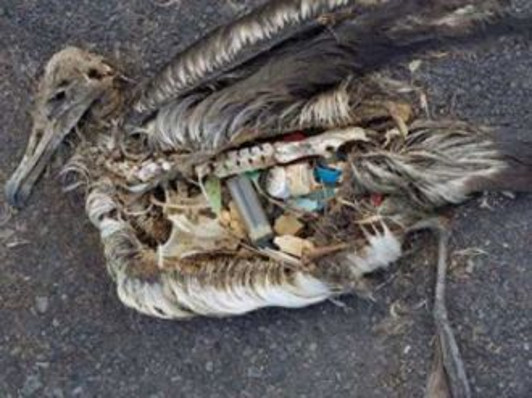
\includegraphics[keepaspectratio=true,width=.5\textwidth]{images/Bird_with_plastic_stomach.jpg}
\caption{The stomach contents of a bird that ate plastic}
\label{fig:plastic-bird}
\end{figure}

\paragraph{Data and approach}
The approach proposed for this project is to use the data set of 40k annotated images.
This data set was constructed from short film clips and annotated by hand.
Figure \ref{fig:plastic-data} shows three images from this data.
The data is split between above and below water, and is annotated with yes/no plastic visible and yes/no marine life visible.

This data set can be used to research what state-of-the-art image techniques are best for solving this problem.
After watching several of the images of the data set, it appears that the `noise' in colour of plastic is much higher than in maritime life.
Therefore I expect that it should be possible to reach a high accuracy on this problem when the three-dimensional colours are used.

The amount of data does not seem enough to construct a Deep learning network, as the supervisor pointed out. Therefore the proposed approach would use a learnt neural net from another project but relearn the last layer of nodes. As Thomas Mensink remarked.

\paragraph{Motivation}
The main reason I chose this project is the possibility to help resolve the plastic soup problem.
After contact with several organisations like Saraswater and the Plastic Soup Foundation they were enthusiastic about this project.
That is why I already collected and annotated a data set.
Besides that my interest and knowledge in Image Recognition from the bachelor courses would help in this project.

\begin{figure}[h!bt]
\centering
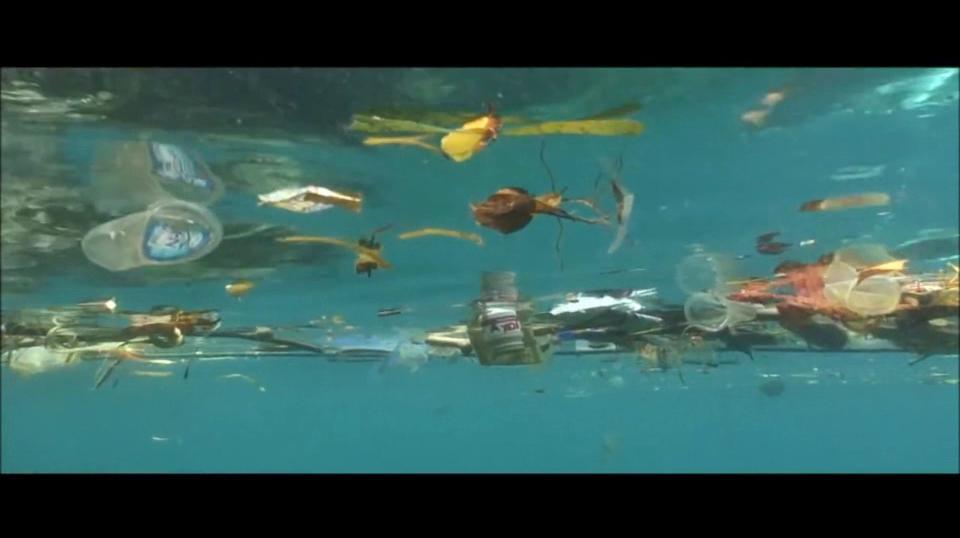
\includegraphics[keepaspectratio=true,width=.5\textwidth]{images/10947_01.jpg}\\
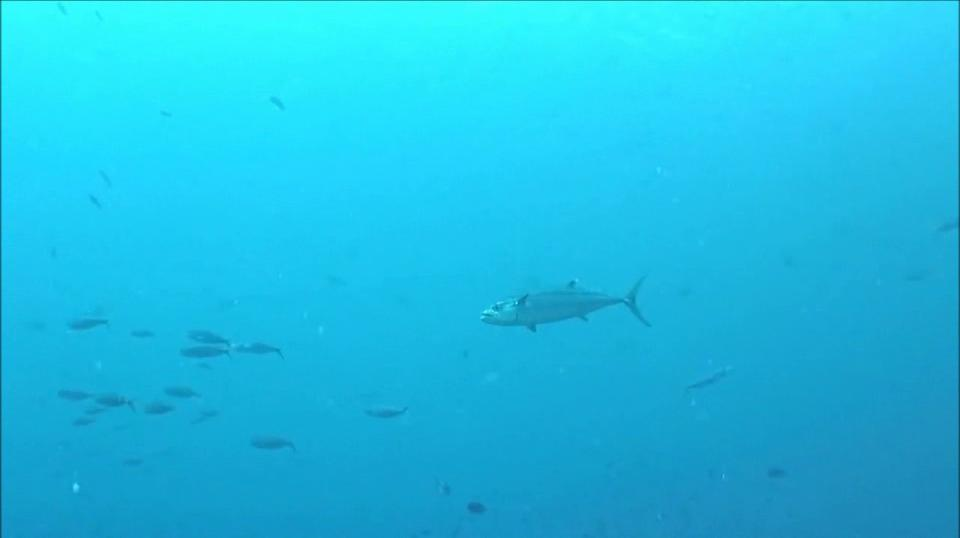
\includegraphics[keepaspectratio=true,width=.5\textwidth]{images/19358_10.jpg}\\
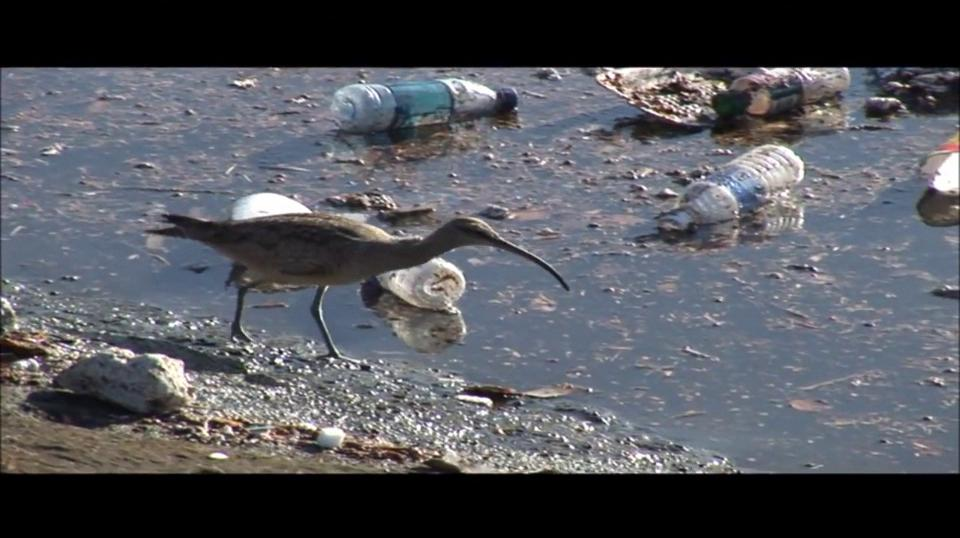
\includegraphics[keepaspectratio=true,width=.5\textwidth]{images/9077_11.jpg}
\caption{Images from the data set. Width plastic (top), width marine life (middle) and width both (bottom)}
\label{fig:plastic-data}
\end{figure}

\vfill
\bibliographystyle{abbrvnat}
\bibliography{Tex_sources/bib}
\end{document}

In this document I will apply for the project that will use Visual Recognition to conserve nature.
An environmental problem that a friend of mine is working on is the Plastic Soup.
Large amounts of plastic waste end up in the world's oceans and have a big inpact on the sea-life.

Saraswater, the organisation my friend works for, is developing ships that `scoop' the plastic out of the water.
I would like to use this project to start automatise this clean-up.
If an autonomous agent could detect from cameras where the plastic is, the ships could be controlled by this agent to clean it up.

My approach would be to use an annotated data set of images, gathered from several organisations that want to solve the Plastic Soup Problem.
I have a data set that contains 16k images from above water and 25k images from below water on which floating plastic, swimming fishes or both are visible.
From this data I will research which state-of-the-art algorithms are fit for this problem and try to optimise them.

Not only does this project fit me for my interest in the problem and the possession of a usable data set, or the knowledge and interest in Image Recognition Leo Dorst gave me but also the fact that I expect this project to benefit from creativity, and as my colleagues could tell, I have a lot of that.

From my point of view after watched several of the images of my data set, the `noise' in colour of plastic is much higher than in maritime life.
Therefore I expect that it should be possible to reach a high accuracy on this problem.